\documentclass[11pt]{article} % use larger type; default would be 10pt
\usepackage[utf8]{inputenc} % set input encoding (not needed with XeLaTeX)

%%% BEGIN Article customizations

%%% PAGE LAYOUT
\usepackage{geometry} % to change the page dimensions
\geometry{a4paper} % or letterpaper (US) or a5paper or....
% \geometry{margin=1in} % for example, change the margins to 2 inches all round
\usepackage[parfill]{parskip} % Activate to begin paragraphs with an empty line rather than an indent

%%% FIGURES
\usepackage{graphicx} % support the \includegraphics command and options
\graphicspath{{../FIGURES/FIGURE_PDFS/}}

%%% PACKAGES
\usepackage{booktabs} % for much better looking tables
\usepackage{array} % for better arrays (eg matrices) in maths
\usepackage{paralist} % very flexible & customisable lists (eg. enumerate/itemize, etc.)
\usepackage{verbatim} % adds environment for commenting out blocks of text & for better verbatim
\usepackage{subfig} % make it possible to include more than one captioned figure/table in a single float
\usepackage{lscape}
% These packages are all incorporated in the memoir class to one degree or another...

%%% HEADERS & FOOTERS
\usepackage{fancyhdr} % This should be set AFTER setting up the page geometry
\pagestyle{fancy} % options: empty , plain , fancy
\renewcommand{\headrulewidth}{0pt} % customize the layout...
\lhead{}\chead{}\rhead{}
\lfoot{}\cfoot{\thepage}\rfoot{}

%%% SECTION TITLE APPEARANCE
\usepackage{sectsty}
\allsectionsfont{\sffamily\mdseries\upshape} % (See the fntguide.pdf for font help)
% (This matches ConTeXt defaults)

%%% ToC (table of contents) APPEARANCE
\usepackage[nottoc,notlof,notlot]{tocbibind} % Put the bibliography in the ToC
\usepackage[titles,subfigure]{tocloft} % Alter the style of the Table of Contents
\renewcommand{\cftsecfont}{\rmfamily\mdseries\upshape}
\renewcommand{\cftsecpagefont}{\rmfamily\mdseries\upshape} % No bold!

%%%Bibliography
\usepackage{natbib}
\usepackage{url}

%%% END Article customizations

%%% The "real" document content comes below...

\title{Reproducibility of SNP calling in multiple sequencing runs from single tumors}
\author{Dakota Z. Derryberry, Matthew C. Cowperthwaite, Claus O. Wilke} 


\begin{document}
\maketitle

\section*{Abstract}

We examined 55 technical sequencing replicates of Glioblastoma multiforme (GBM) tumors from The Cancer Genome Atlas (TCGA) to ascertain the degree of repeatability between sequencing runs of a single tumor, and to determine if the similarity between the two is increased or decreased by SNP-callers like SomaticSniper. To investigate this, we measured the extent of the overlap between two technical sequencing replicates from the same tumor (n=55), that is how many specific point mutations were found by both sequencing runs, using strictly computational means. We further examined whether the degree of overlap was higher or lower when using the SNP calling program SomaticSniper.  We found that about half of the putative mutations found in one sequencing run of a given sample are also found in the second, and that this percentage remains steady throughout orders of magnitude of variation in the total number of mutations called (50 to 7000). We further found that using a SNP caller removes the overlap completely, probably because the SNP caller weeds out such a high percentage of the total putative mutations (between 95\% and 100\%). We conclude that there is variation in the frequency of mutations in GBMs, and that some parts of the SNP caller function more accurately than others.

\section*{Introduction}

The past six years have seen an explosion of data in cancer genomics, an effort led by TCGA, an archive of publicly-available data that includes sequencing of paired tumor-normal samples from a single patient for thousands of tumors \citep{TCGA-GBM, TCGA-GBM-13}. TCGA's database includes hundreds of samples of each of several tumor types, including 580 and counting samples alone of Glioblastoma multiforme (GBM), the most common and deadly primary brain tumor. GBM has a median survival of 14 months and a 5-year survival of ~5\%, and prognosis for patients with this disease remains poor despite significant research investment, due to the difficulty of surgical resection and the limited number of effective chemotheraputics \citep{GBM-stats}. In an effort to improve patient outcomes, TCGA and other groups \citep{Parsons} have used large scale genomic data to discover which genes and pathways are mutated in GBM \citep{pathways}, discover different GBM subtypes \citep{subtypes}, and develop a variety of computational models to find GBM driver mutations \citep{drivers}.

Despite widespread use of TCGA data in these and other research efforts, and significant monetary investment in collecting the data, there has been very little investigation of the best way to sequence the 580+ paired tumor/normal samples in the TCGA GBM database. Most samples in the database include, at a minimum, whole exam sequencing of both the tumor and a matched blood sample at a coverage depth of between 8X and 80X, usually around 10--15X in the blood and 20--50X in the tumor. This is low, but similar to the 30X recommended for variant calling by the Broad Institute Introduction to NGS. However, we can find no research looking at the accuracy of variant calling at this or any sampling depth, for common or rare variants, in normal or cancerous tissue. Given that cancer is thought to be genetically heterogenous \citep{heterogenous1, heterogenous2}, and that rare variants in GBM may be functionally important \citep{rare}, we think that some inquiry into the accuracy and precision of standard cancer sequencing methods is warranted. 

In this paper, we begin this inquiry with two simple questions: Given two technical sequencing replicates of a single tumor, how similar are they? Does SNP-calling software increase or decrease the degree similarity? We answered these questions using data from TCGA, which includes 55 GBM tumors that were sequenced twice, once each with (i) the standard WGS protocol, and (ii) an additional amplification step before library prep, which we refer to as the WGA protocol. For each of these 55 samples, we compared the somatic variants found in the WGS and WGA replicates, before and after analyzing the variants using SomaticSniper \citep{SomaticSniper}. We found significant overlap (around 50\%) between technical replicates, but also significant differences. As expected, the additional amplification step in the WGA protocol versus the WGS protocol added some putative mutations to the sample, so that on average these replicates had (i) more putative mutations, and (ii) a smaller percentage overlap between replicates. Still, the number of mutations in the WGS replicates only varied by orders of magnitude, from under 100 to almost 10,000. Contrary to expectations, the quality of results (measured by the percentage overlap between technical replicates) did not decrease with increasing numbers of mutations, suggesting real variation in mutation frequency between samples. This may be in part due to know mutational hotspots in some tumors \citep{Karen}. Using SomaticSniper and some custom protocols to analyze the likelihood that individual variants were true positives (actual somatic mutations in the tumor, and not sequencing or analysis errors or various sorts) was unsuccessful, because almost no putative SNPs were identified as probably SNPs.

\section*{Results}

\subsection*{Just how similar are two iterations of sequencing the same tumor?}

% Experiment: size of overlap (figures 3 and 4)
%(a) a brief (one sentence to one paragraph) summary of what you did and why
%(b) a description of what you found carrying out this experiment

DNA sequencing is not error-free. Error is introduced by mis-called bases in sequencing runs, and by mis-aligned bases during sequence analysis \citep{seqerror}. Loss of heterozygosity also occurs in sequencing, if only one allele of a polymorphic site is amplified. Cancer DNA is highly heterogenous, which makes for an additional source of error: a mutation present in only some tumor cells may or may not be present in a sample that is sequenced, so that a partially penetrant mutation may appear fixed or not at all. In general, we would like to know how often these error occur. One way of investigating would be to use PCR to verify each individual mutation, but this method is expensive and time consuming. A cheaper alternative would be to sequence the tumor multiple times, and look at the similarity between the iterations. Theoretically, any mutation fixed throughout the tumor should appear in all replicates, while errors due to (i) sequencing errors, (ii) amplification errors, or (iii) alignment errors would not. (Incompletely penetrant mutations would also not be fixed in all samples, so this method does not address the difficulty of calling low-frequency variants in tumors.) This is the method used in most biological sequencing experiments--but not generally in cancer genomics, presumably due to the expense of sequencing multiple replicates for each of the hundreds of samples necessary for cancer genomics research. Still, even if researchers cannot verify every mutation or sequence multiple replicates for each tumor, it would be useful to know about what percentage of called mutations would or would not likely appear in additional sequencing replicates.

TCGA's GBM data set includes 2 technical replicates each of 55 tumors. In this case, the technical replicates are not identical; one includes an additional amplification of DNA before preparing a library; we refer to this replicate as the WGA replicate, and the other as the WGS replicate. Despite this difference, we can still assume that any mutation fixed throughout the tumor should appear in both replicates, and so those putative mutations appearing in both replicates are more likely to be real, fixed somatic variants than those found in only one replicate. We further hypothesized that the WGA samples should have a greater number of amplification errors, and thus there should be more putative SNPs per sample, than the corresponding WGS samples. 

For each patient (n=55), we called mutations in both technical replicates and the patient's blood sample using the same computational pipeline (see Figure 1 and Methods): we downloaded TCGA bamfiles with CGHub \citep{CGHub}, re-generated fastq files with picard \citep{picard}, re-aligned the fastq files to hg19 with bwa \citep{bwa}, performed indel re-alignment and base recalibration with GATK \citep{GATK}, and finally called somatic mutations with SomaticSniper \citep{SomaticSniper}. We then compared the lists of putative SNPs generated by the WGS and WGA bamfiles for each patient, and calculated the length of each list and the length of the overlap, or intersection, between the two lists (Figure 2). We further calculated the percent of the WGA list that overlapped with the WGS list and the percent of the WGS list that overlapped with the WGA list. We found that the number of mutations found in one replicate correlated strongly with the number of mutations found in the other, though as expected the WGA replicate, with the additional amplification step, had slightly more mutations (Figure 3). We further found that the percent overlap between the two samples, calculated by $WGA \cap WGS/WGS$ for WGS replicates and $WGA \cap WGS/WGA$ for WGA replicates, was fairly consistent, mostly between 20--40\% in WGA replicates and mostly between 40--60\% in WGS replicates. As expected, the distribution was narrower and taller in the WGS replicates, because on the whole the WGA samples had more amplification errors than the WGS samples (Figure 4).

% Experiment: number of mutations (figure 5)
%(a) a brief (one sentence to one paragraph) summary of what you did and why
%(b) a description of what you found carrying out this experiment
Although the percent overlap in WGS and WGA samples remained fairly constant, and the number of possible mutations in WGS and WGA lists was correlated, the exact number of putative mutations varied across samples by orders of magnitude (less than 100 to over 10,000). Different cancers mutate at different rates: some pediatric cancers have very few mutations \citep{RB2hit, pediatric}; other tumors show a mutator phenotype, leading to vastly more mutations, usually resulting from errors in DNA repair pathways \citep{mutator}. GBM specifically is thought to have a relatively low mutation rate \citep{Parsons, TCGA-GBM-13}, and while the majority of our samples had low mutation frequencies in line with this theory, several samples also had mutation frequencies an order of magnitude greater. One possible explanation is a degraded DNA sample, or bad data. If this were the case, we would expect the percentage of the overlap between replicates (a measure of data quality) to decrease with the overall number of putative mutations. We found no correlation between the number of putative mutations and the percentage of the sample that was overlapping (Figure 5). That the percentage overlap does not vary with the number of putative mutations in either replicate suggests that some samples may simply have a higher mutation rate than others, or indeed than is generally supposed in GBM.

\subsection*{Does SNP-calling software increase or decrease the degree similarity between replicates?}

% Experiment: which filters do what (figures 4 and 5) % Experiment: those two filters are different (figures 6 and 7)
%(a) a brief (one sentence to one paragraph) summary of what you did and why
%(b) a description of what you found carrying out this experiment
The aim of sequencing tumors is generally to find somatic mutations, those mutations that arise in a tumor and are not present in the rest of the organism. To do this, researchers sequence a patient's tumor and blood and align the two to each other; Differences between the two sequences are putative somatic mutations. Because sequencing is not error free, and because a patient's blood tissue might also have somatic mutations different from the tumor, not all of the putative somatic mutations are mutations, and some method of distinguishing true somatic mutations from sequencing and other errors is needed. If possible, this is done by individually validating each putative mutation with PCR; however, due to restraints on time and money, as well as the amount of tumor tissue available and its purity, this is often not possible. In this case, computational algorithms that attempt to distinguish somatic mutations from germ line mutations and sequencing error may be employed \citep{SomaticSniper, mut_calling}. 

Software platforms to distinguish somatic mutations from germ line mutations and sequencing error are plentiful, and each one typically employs multiple methods to identify true positive mutations. SomaticSniper, the platform used in this research, uses several probabilistic calculations based on features of the dataset to sort out true putative mutations from false ones \citep{SomaticSniper}. Another example, the GATK QualityScore, calculates the probability that a mutation is a true mutations based on features of the reads \cite{GATK}. In this paper, we used eight different methods, or filters, to identify somatic mutations, summarized in Table 1. The first three are the quality scores generated by the GATK and SomaticSniper (we simply remove from the dataset anything that fails to meet these thresholds). The last five we coded ourselves in Python. Each of these five filters represents a quality of the data or putative mutation that is generally thought to indicate that it is probably a false positive.

Our initial question was, does filtering the data increase or decrease the percentage of the sample that is overlapping between the two technical replicates? Put another way, does filtering out putative somatic mutations with these features increase or decrease the proportion of true somatic mutations in the remaining dataset? We found that after removing putative mutations tagged by any of the eight filters, the number of putative mutations per replicate decreased from 50--10,000 to 0--14. The size of the overlap between technical replicates decreased to 0--2 per sample, with 0 as the mode, so the overall percentage also decreases. We concluded that running all the filters on the data, in the absence of any other verification method, was counterproductive, because it removed all of the signal (as well as the noise). 

We next looked at the individual effects of each of the five filters that we coded, and one of the SomaticSniper filters (Variant Allele Quality, or VAQ). We first looked at the total number of putative SNPs removed by each filter (Figure 6). We found that different filters removed different numbers of mutations, and that the lion's share of mutations were removed by the VAQ and LOH filters, each of which removed 200 or more putative SNPs on average. Three other filters, those removing overlap with dbSNP and mutations within a 10 bp window of other mutations, also removed around 50--100 mutations each per sample (Figure 6). The final filter, which removed putative SNPs with less than 10\% coverage of the alternate allele, removed 0--1 putative SNPs on average, but did on occasion remove as many as 50. 

We next asked how many of the mutations removed by each filter were mutations present in the overlap between technical replicates, and how many were in just one sample? Put differently, what percentage of putative SNPs removed by a given filter were in the category more likely to be true positives (overlap), versus the category less likely to be true positives (only one replicate). To answer this, we graphed the percent of the overlap only (per sample) that was filtered by each of the six filters (Figure 7). We found that the three filters removing overlap with dbSNP and other putative mutations removed almost none or none of the overlap, despite removing 50--100 putative mutations on average. In contrast, the VAQ filter (specific to SomaticSniper) and the LOH filter each removed about half of the overlap between replicates (Figure 7). Thus, our evidence suggests that the filters removing overlap with dbSNP and putative mutations near other putative mutations are preferentially removing false positives, but the filters removing low VAQ and LOH are less discriminatory. 

%% this is figures 8 and 9, which need to be added to the document and explained now...
Finally, we asked whether the VAQ and LOH filters, responsible between them for removing most of the overlap, were removing the same or different putative SNPs in each sample. We plotted the percent of the overlap filtered out by the LOH filter against the number of putative mutations in the overlap (Figure 8), and the percent of the overlap filtered out by the VAQ filter against the number of putative mutations in the overlap (Figure 9). We found opposite trends: the percentage filtered out by VAQ decreased, and the percentage filtered out by LOH increased, with increasing length of overlap. We concluded that the LOH and VAQ filters were not removing the same putative mutations. 

\section*{Discussion}

GBM, primary brain cancer, is an evolutionary process by which mutations arise in glial cell lines and these mutated cells and their lineages co-opt the surrounding tissue and systems to the detriment of the organism of the whole. Treatment for GBM is difficult and has poor outcomes \citep{GBM-stats}, but could hopefully be improved by a more complete understanding of the somatic mutations present in GBM. Large-scale sequencing projects, like TCGA, make cancer sequencing data available to many researchers. This data is enormously valuable to the research community, but the accuracy and reproducibility of these data are unknown, and knowing them could only increase the utility and value of the data. We make a first pass at evaluating the accuracy and repeatability of the data by comparing 55 technical replicates in the TCGA GBM dataset.  

We looked at the similarity between technical GBM genomic sequencing replicates for 55 samples in TCGA. We found that on average, about half of the putative mutations in the raw data for the WGS replicate (no amplification before library preparation) and about a third of those in the WGA replicate (with amplification before library preparation) were present in both replicates. The number of mutations present in both replicates was anywhere between 50 and 5,000 putative mutations. We found that the high number of putative somatic mutations in some, but not all, of the patient samples was repeatable across technical replicates. Further, samples with a higher frequency of putative mutations had equally similar technical replicates to those samples with a lower frequency of putative mutations. This suggests the possibility that a higher mutation frequency could be a feature of a subset of GBM tumors and not a data artifact.

Filtering the raw computational data using both custom filters and those in the software SomaticSniper eliminated more than half of the total number of putative mutations in all 110 samples, including most or all of those present in both replicates.  Of the six filters whose individual effects we examined, only two, those that removed Loss of Heterozygosity (LOH) mutations and putative mutations with low VAQ (calculated by SomaticSniper), removed primarily mutations that found in both technical replicates. Combined, the two removed most or all of those mutations present in both replicates. Despite this, two still appeared to remove different sets of mutations. Of the remaining four, only three removed any appreciable number of putative mutations from the sample, and each of these preferentially removed mutations present in only one technical replicate. Two of these three filters, those removing putative mutations within a 10 bp window of other putative mutations or within a 10 bp window of a putative indel, recognized a feature (clustered mutations) that suggested a local problem with the reads or alignment, and removed this data from consideration. The third removed overlap with dbGaP.  Our analysis suggests that these three filters are useful, and do clean up the purely computational data in a meaningful way. By contrast, it may be more useful to discard the two filters that removed principally data from the overlap of the two replicates. Of these, one, VAQ is built into SomaticSniper. The second removes loss of heterozygosity (LOH) mutations. Multiple sources suggest that LOH mutations may be essential to cancer \citep{LOH}. This, along with the data presented here, makes a strong argument for retaining these mutations in functional analyses rather than excluding them.

Several factors limit the conclusions we may draw from this analysis. First, in this analysis we use repeatability between technical overlaps (being in the WGS and WGA samples) as a measure of confidence in a putative SNP. This metric is potentially problematic for three reasons: (i) cancer is highly heterogeneous, and so a legitimate somatic SNP might show up in one replicate and not another; (ii) if the DNA sample is degraded to some extent, due to surgery conditions or some other factor out of the hands of the sequencing center, the same errors may appear in both replicates; and (iii) a putative mutation that is in both samples may be a somatic mutation that arose before the tumor \citep{pre-tumor-muts}. Although repeatability does not and could not perfectly measure confidence that a putative mutation is a somatic mutation, it does make it more likely. Having an independent measure of the confidence in SNP calls (repeatability), even an imperfect one, can help us gauge the accuracy of other measures (filtering).  In this sample, we have shown that while some filters remove primarily putative SNPs in only one of two replicates (more likely to be false positives), two filters, VAQ and LOH, remove most of the overlap (more likely to be true positives). While our results suggest that VAQ and LOH filters are probably removing some true positives, that does not preclude them removing false positives. Therefore, if we remove these filters, we may retain more true positives, but we also retain more false positives. 

Second, we looked at results from one SNP caller. There are many more equally widely used SNP callers available, which might do better or worse than the one we have chosen here. Additionally, we have shown that the VAQ filter does not avoid putative mutations in both replicates; however, we did not look at the SomaticScore, also a feature of SomaticSniper, or the GATK quality score. 

We have shown that there is significant overlap between technical replicates of whole exome sequencing in the TCGA GBM dataset, comprising about 50\% of putative SNPs in WGS samples and about 30\% in WGA samples. This effect remains even at a high number of putative SNPs, suggesting that some GBMs may have significantly more somatic mutation than others. While PCR remains the gold standard for distinguishing true positives from false positives in sequencing, we looked at the effects of six strictly computational filters on the putative mutations in each technical replicate and the overlap between them, for all 55 samples. We found that some filters remove principally those mutations found in one sample or the other, while other filers remove primarily those in the overlap. We suggest using just the first set in the future, when mutation validation by PCR is not an option.

\section*{Methods}

\subsection*{Data and back-end processing}

All sequence data came from The Cancer Genome Atlas (TCGA) Research Network's Glioblastoma multiforme (GBM) data set \citep{TCGA-GBM}. We downloaded three bamfiles for each of 55 patients using CGHub \citep{CGHub}. For each patient, data consisted of one bamfile taken from blood DNA, and two bamfiles from tumor DNA, one for each technical replicate. In each case, the only difference in data collection for the two sets of tumor DNA was whether or not an amplification step was performed prior to building a library \citep{TCGA-GBM}. 

We created a pipeline for backend processing of all TCGA bamfiles, summarized in Figure 1, with commands given in Table 2. The custom python code to connect the pipeline is available in a public 
git repository (\texttt{https://github.com/clauswilke/GBM\_genomics}). Our pipeline first regenerated fastq files (original reads) from the TCGA bamfiles, which were aligned to hg18, using picard \citep{picard}. Next, we used BWA \citep{bwa} to align the fastq files to hg19, and samtools \citep{SAMtools}to sort, index, clean, and de-duplicate the new bamfile. We used GATK \citep{GATK} to do indel realignment and base recalibration, according to the standards best practices for genomics data \citep{best-practices}. Finally, we predicted somatic variants with SomaticSniper \citep{SomaticSniper}, with the output given in VCF format.

\subsection*{Filtering and data analysis}

After generating a VCF file will all of the putative somatic variants for each replicate of each sample, we used custom python code (available in public git repository) to list the putative mutations in each VCF, and to calculate the overlap between technical replicates. We then filtered the lists of putative SNPs according to the eight filters described in Table 1, using a combination of command line options and custom python code (available in a public git repository). The eight filters were enacted as follows: 

\begin{enumerate}
\item (GATK) The GATK quality score is automatically generated by GATK; GATK recommends discarding all putative mutations with a quality score below 40, which we did using the command line option \texttt{-q 40} when we called SomaticSniper (for the exact command, see Table 2). We did not at any point consider putative mutations removed by this filter, and did not consider its individual action. 
\item (SS) The SomaticScore is a similar metric calculated by SomaticSniper. As recommended, we removed from consideration all putative mutations with a SomaticScore below 40 by using the command line option \texttt{-Q 40} when we called SomaticSniper (for the exact command, see Table 2). We did not at any point consider putative mutations removed by this filter, and did not consider its individual action. 
\item (VAQ) The Variant Allele Quality (VAQ) score calculated by SomaticSniper is a third measure of this type. SomaticSniper recommends discarding putative mutations with a VAQ below 40, which we accomplished using a custom python script available in the public git repository. This recommendation is discussed in the Results and Discussion.
\item (LOH) It is general (but not universal) practice to disregard Loss of Heterozygosity (LOH) in large scale cancer genomics, because it to easily results from sequencing errors. We were able to exclude LOH variants using a custom python script available in the public git repository. This recommendation is discussed in the Results and Discussion.
\item (10bp-SNP) It is universal or near universal practice to exclude variants within 10 bp of another putative somatic variant, because this often indicates an error in reads or sequence alignment. We were able to exclude 10bp-SNP variants using a custom python script available in the public git repository. This recommendation is discussed in the Results and Discussion.
\item (10bp-INDEL) It is universal or near universal practice to exclude variants within 10 bp of a putative indel, because this often indicates an error in reads or sequence alignment. We were able to exclude 10bp-INDEL variants using a custom python script available in the public git repository. This recommendation is discussed in the Results and Discussion.
\item (dbSNP) It is universal or near universal practice to exclude variants that overlap with dbSNP, because this often indicates an amplification error and not a true somatic variant. We were able to exclude dbSNP variants using a custom python script available in the public git repository. This recommendation is discussed in the Results and Discussion.
\item ($<10\%$) It is universal or near universal practice to exclude variants when the alternate allele coverage is less than 10\%, because this often indicates sequencing error. We were able to exclude $<10\%$ variants using a custom python script available in the public git repository. This recommendation is discussed in the Results and Discussion.
\end{enumerate}

We used the same or substantially similar python scripts to calculate and compare the overlap between technical replicates before and after filtering. These scripts are also available in the public git repository. We plotted all data and did all statistics with standard plotting and statistics functions in R \citep{Rsoftware}. This code is also available in the public git repository.  

%\section*{}

\bibliography{TCGA_bib}
\bibliographystyle{peerj}

\section*{Tables and Figures}

%% Filters table
\begin{landscape}
\begin{table}
\caption{\textbf{SNP prediction filters.} This table shows the various methods (filters) used to predict which differences found in tumor bamfiles relative to blood bamfiles are real somatic variants, as opposed to sequencing error or other variants.}
\begin{tabular}{ p{2.25cm} p{4.25cm} p{14cm} }
	filter & software & purpose \\
	\hline
	GATK & GATK & Removes putative SNPs with GATK quality scores less than 40 (as part of the GATK processing, with indel realignment and base recalibration) \\
	SS & SomaticSniper & Removes putative SNPs with a SomaticScore less than 40 \\
	VAQ & SomaticSniper & Removes putative SNPs with SomaticSniper Varaint Allele Quality scores less than 20 \\
	LOH & SomaticSniper, python & Removes putative SNPs that are identified as loss of heterozygosity \\
	10bp-SNP & python & Removes putative SNPs located within a 10 bp window of any other putative SNP \\
	10bp-INDEL & python & Removes putative SNPs located within a 10 bp window of indels \\
	dbSNP & python & Removes putative SNPs that overlap with dbSNP coverage \\
	$<$10\% & python & Removes putative SNPs if, in the tumor data, the percentage of reads covering the site with the alternate allele is less than 10\% \\
\end{tabular}
\end{table}
\end{landscape}

%% Data processing commands table
\begin{landscape}
\begin{table}
\caption{\textbf{Back-end Processing.} This table shows the software packages we used in data processing, what we used each piece of software for, and the command associated with it. The rows are in order of use.}
\begin{tabular}{ p{2.5cm} p{6cm} p{12cm} }
	software & purpose & command\\
	\hline
	picard & regenerate fastq files from bamfile aligned to hg18 & \texttt{java -d64 -Xmx4g -jar SamToFastq.jar I=\$pfx.bam F=\$pfx.1.fastq F2=\$pfx.2.fastq 2$>$\&1} \\
	bwa & align fastq files to hg19 & \texttt{bwa aln -q 30 -t 8 \$hgReference \$fastq $>$ \$fastq.aln.sai} \\
	bwa, samtools & convert aligned fastq files into new bamfile & \texttt{bwa sampe -a 600 -P -r "\$RG" \$hgReference \$fastq1.aln.sai \$fastq2.aln.sai \$fastq1 \$fastq2 | samtools view -bSh -o \$outprefix.bam -} \\
	samtools & sort and index new bamfile & \texttt{samtools sort -@ 16 \$outprefix.bam \$outprefix.sorted 2, samtools index \$outprefix.sorted.bam 2} \\
	samtools & remove duplicate reads from bamfiles & \texttt{samtools rmdup ../\$tumorpfx/\$tumorpfx.out.sorted.bam \$tumorpfx.dedup.bam} \\
	GATK & indel realignment & \texttt{java -d64 -jar \$gatkJar -R \$hgReference -T IndelRealigner -rf BadCigar -I \$tumorpfx.dedup.bam -known \$G1000.Mills -known \$G1000.Phase1.Indels -targetIntervals \$tumorpfx.intervals -o \$tumorpfx.realn.bam} \\
	GATK & base recalibration & \texttt{java -d64 -jar \$gatkJar -nct 8 -T BaseRecalibrator -rf BadCigar -I \$tumorpfx.realn.bam -R \$hgReference -knownSites \$dbSNP -o \$tumorpfx.recal.grp} \\
	samtools & index recalibrated bamfile & \texttt{samtools index \$tumorpfx.realn.recal.bam} \\
	SomaticSniper & call somatic mutations, generate VCF & \texttt{bam-somaticsniper -q 40 -Q 40 -J -s 0.001 -F vcf -f \$hgReference \$tumorbam \$normalbam \$tumorpfx.SS.vcf} \\
\end{tabular}
\end{table}
\end{landscape}

%% Figure 1
\begin{figure}
\centerline{
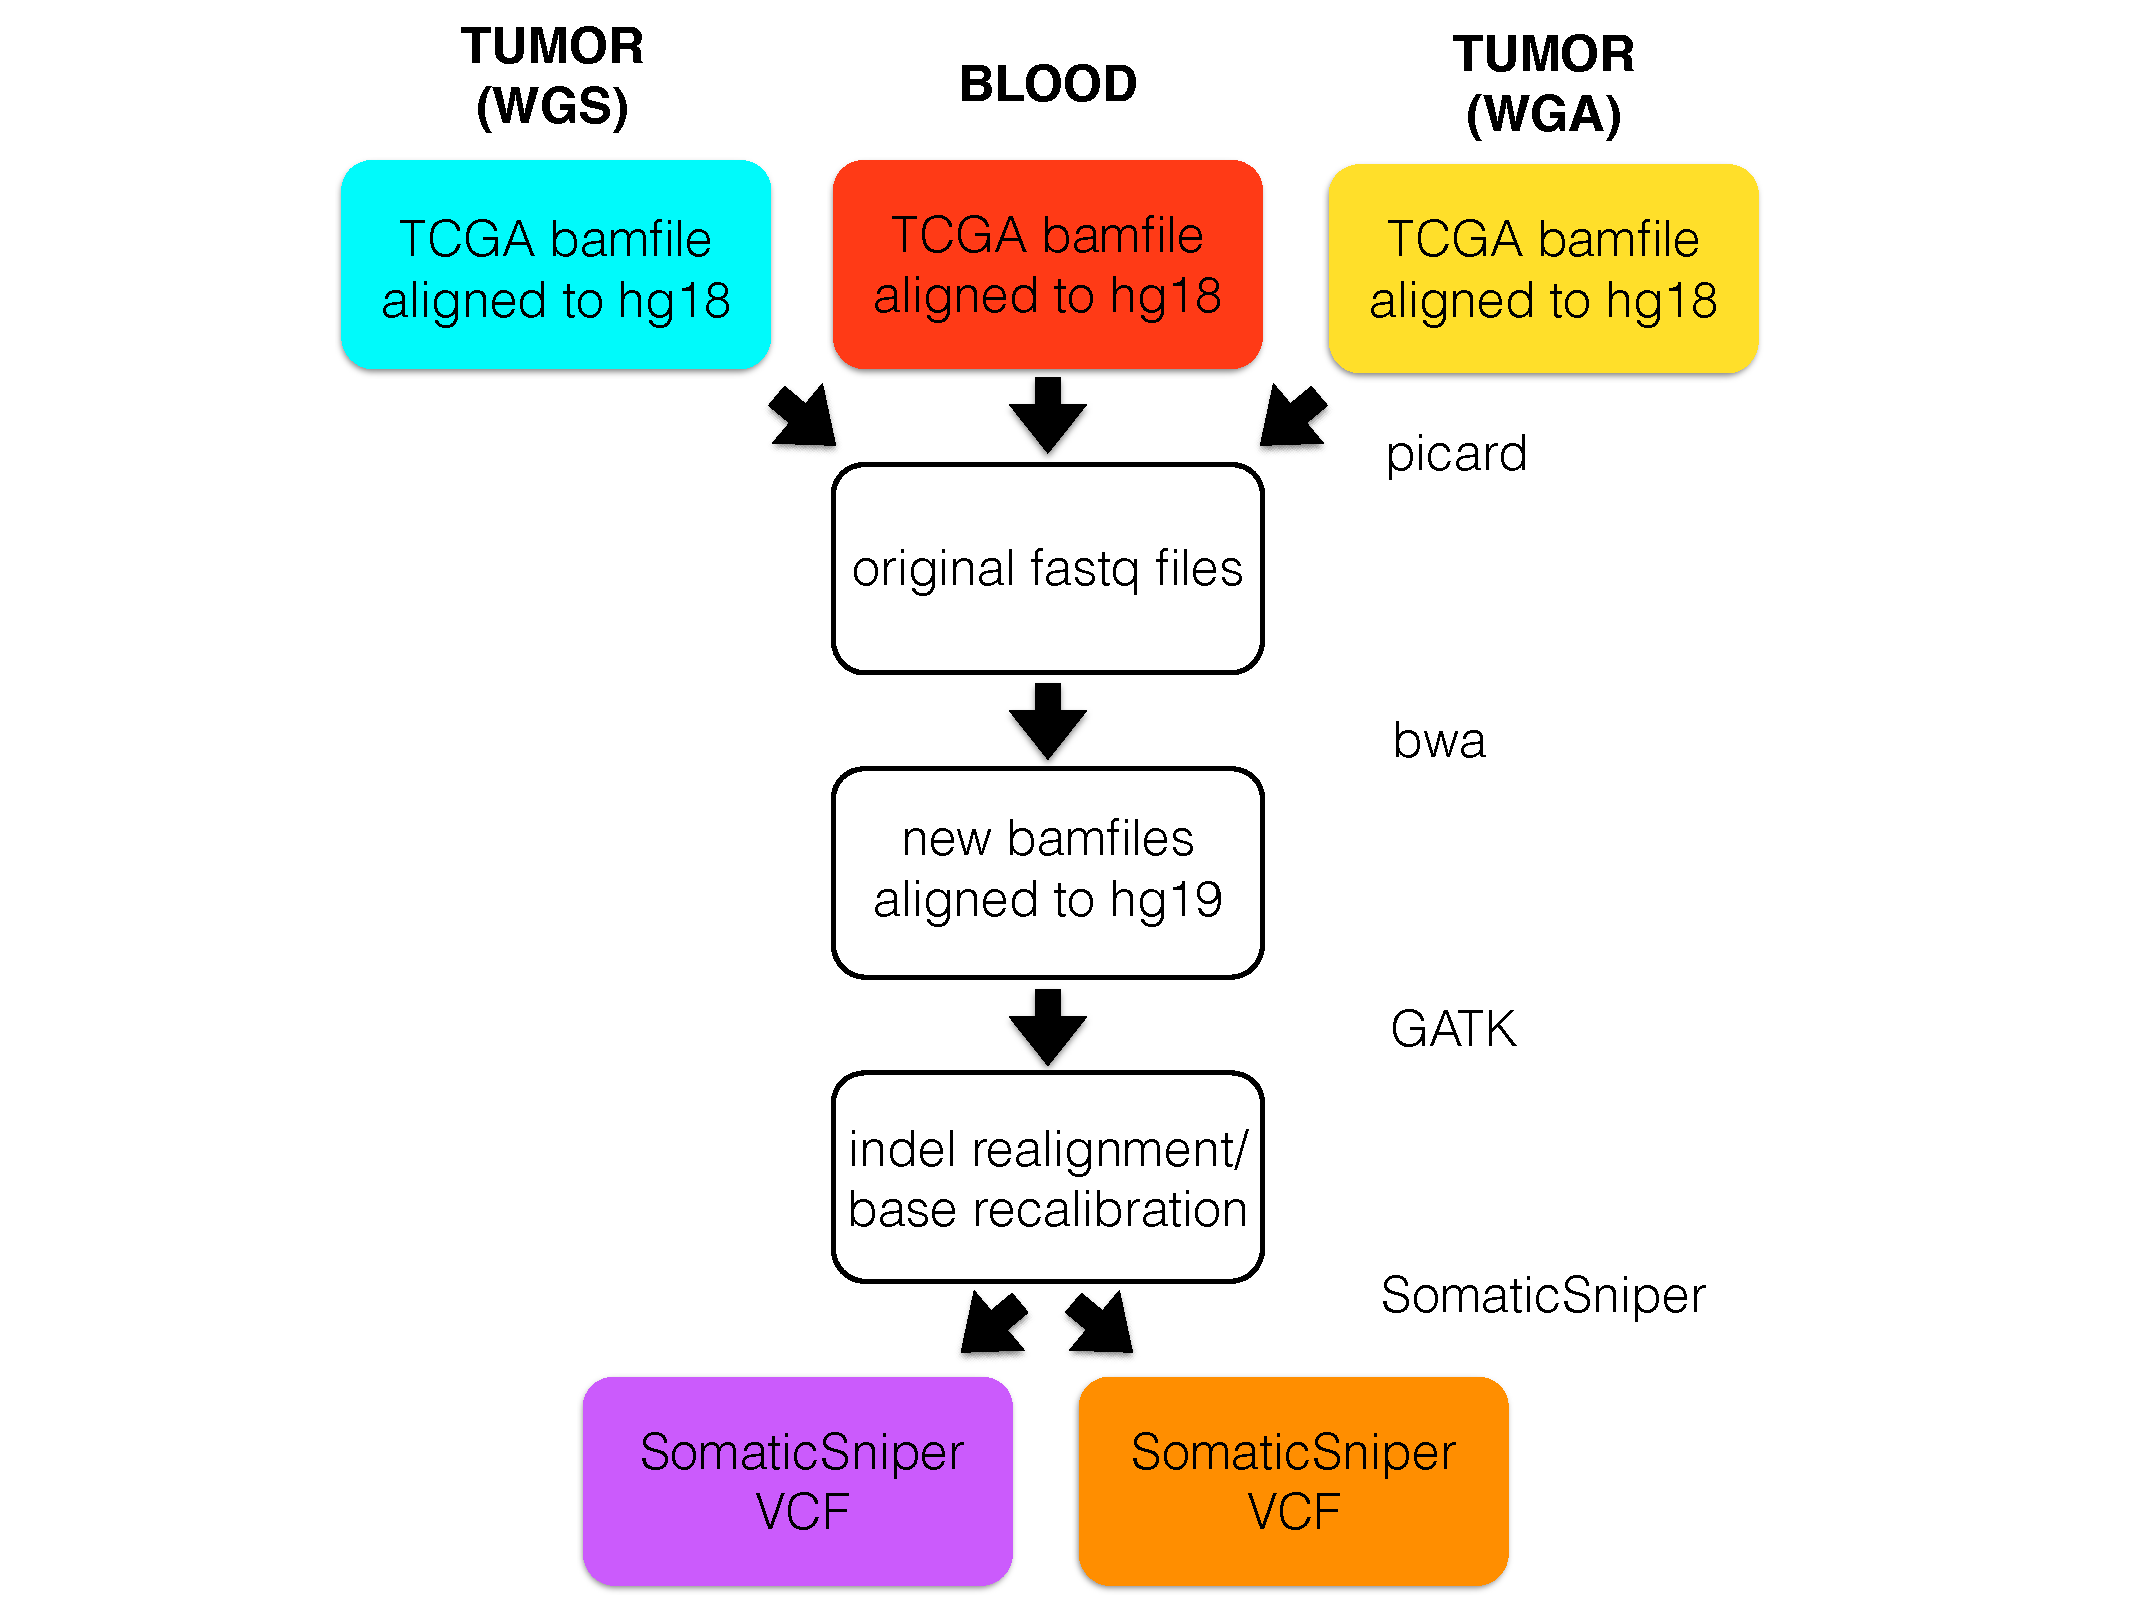
\includegraphics[width=6in]{figure1.pdf} }
\caption{\textbf{Back-end processing pipeline.} For each of 55 patients, we began with a C484 tumor bamfile (WGS), a C282 tumor bamfile (WGA), and a normal bamfile, all aligned to hg18. For each bamfile, we used picard to regerate fastq files, bwa to realign the fastq files to hg19, GATK to recalibrate bases and indels, and SomaticSniper to call somatic mutations.}
\end{figure}

%% Figure 2
\begin{figure}
\centerline{
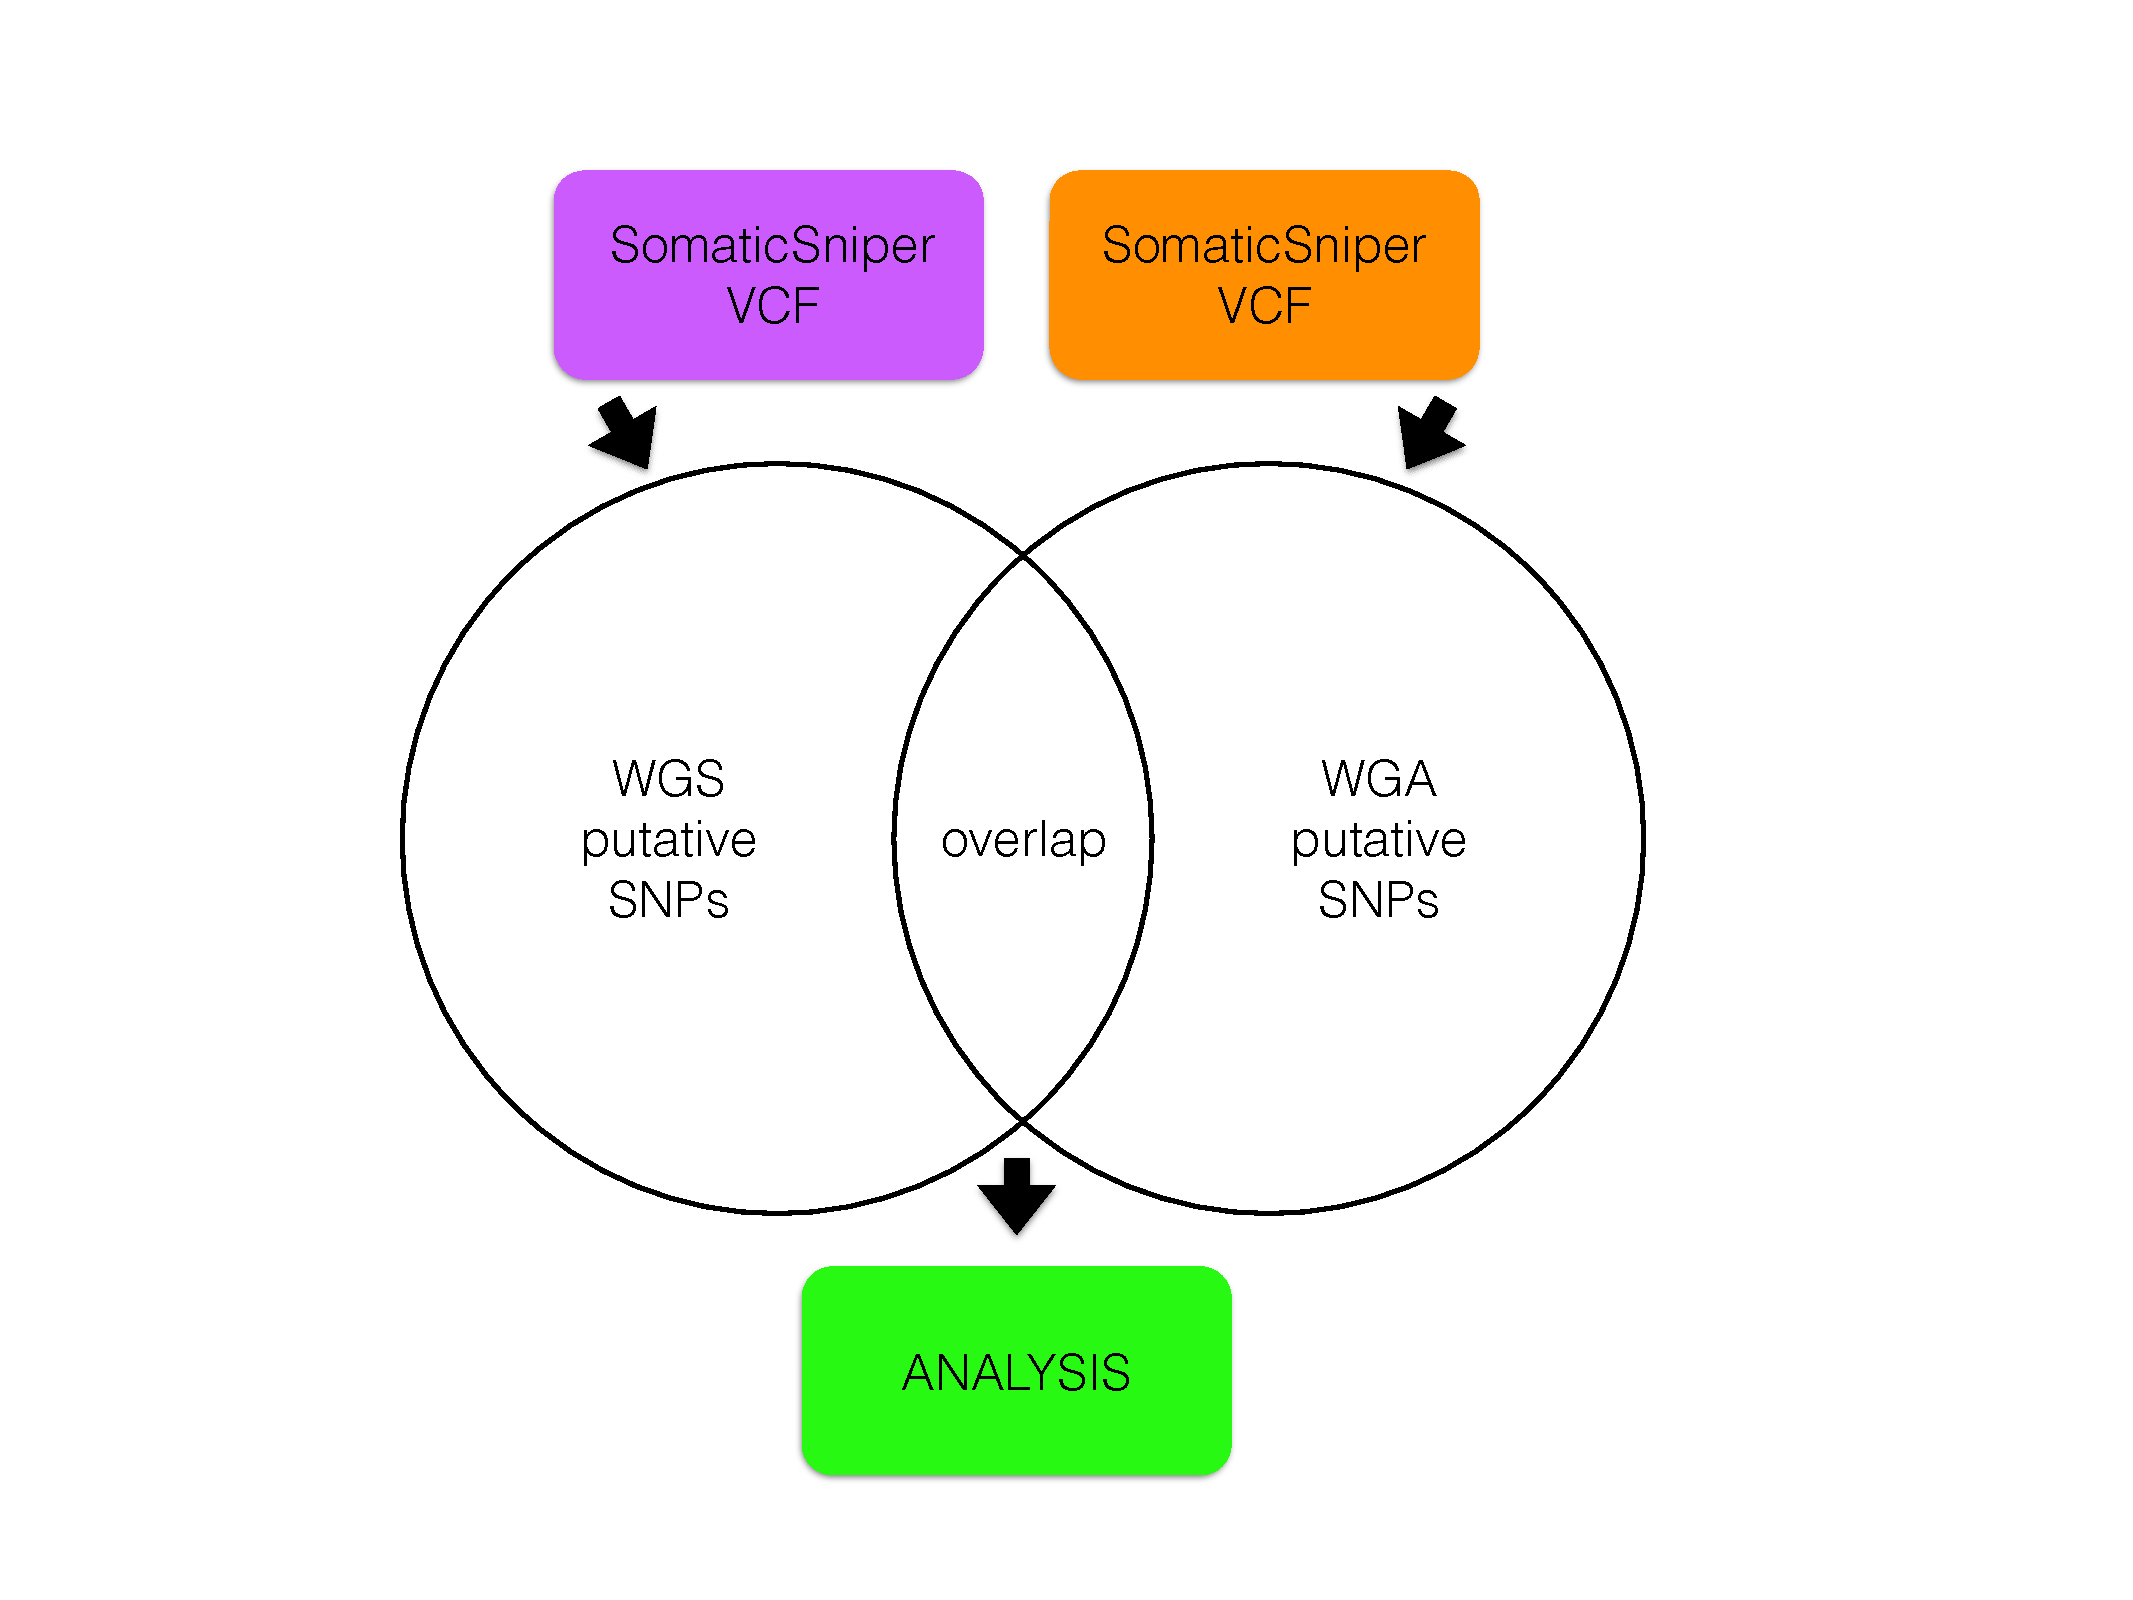
\includegraphics[width=6in]{figure2.pdf} }
\caption{\textbf{Definition of overlap between replicates.} For each sample, we generated a SomaticSniper VCF with putative somatic mutations for each of two replicates. We took the overlap between the two lists for the most likely true positives.}
\end{figure}

%% Figure 3
\begin{figure}
\centerline{
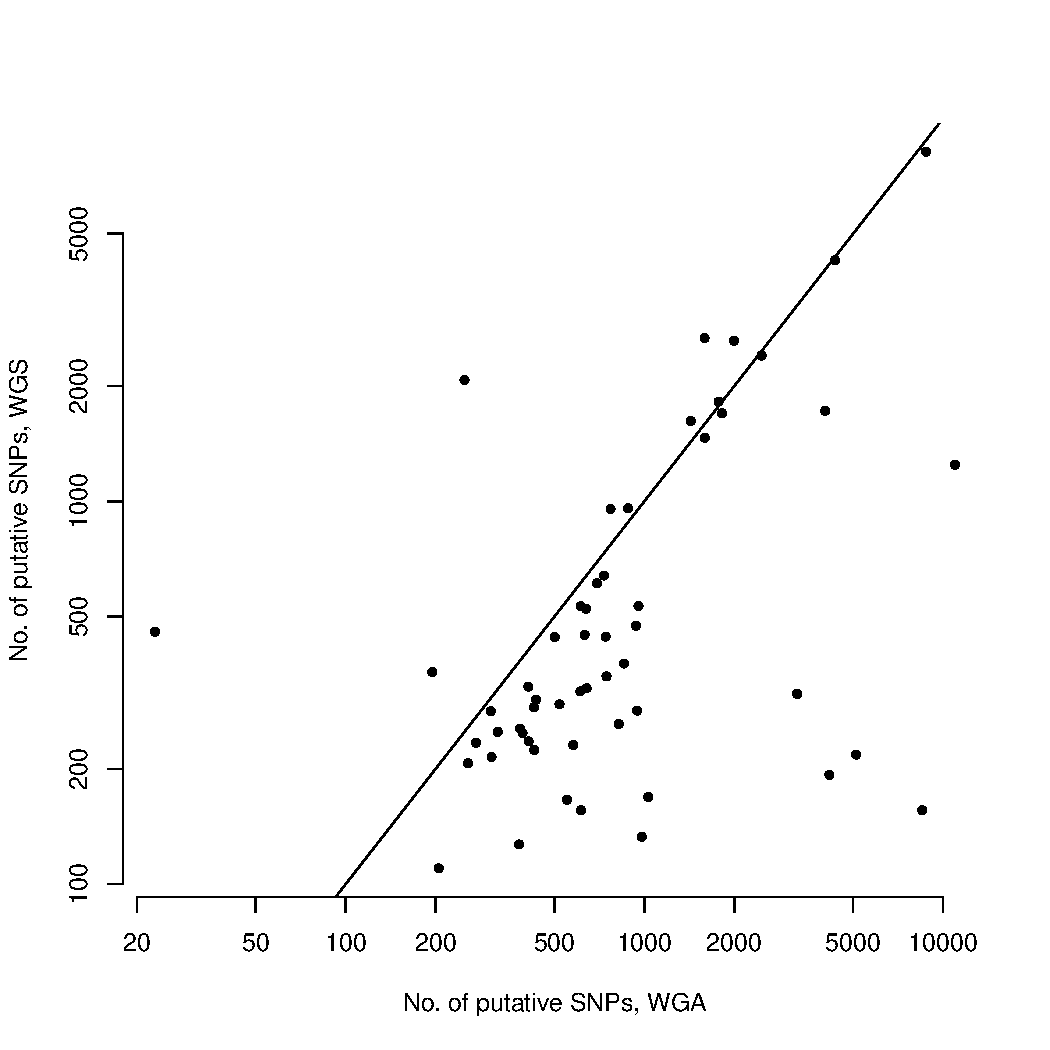
\includegraphics[width=5in]{C282_v_C484.pdf} }
\caption{\textbf{Number of putative SNPs in WGS v. WGA, as called by SomaticSniper.} Each point is a patient. The line is $y=x$, so points falling below the line agree with the hypothesis that an additional amplification step produces more sequencing errors in a sample.}
\end{figure}

%% Figure 4
\begin{figure}
\centerline{
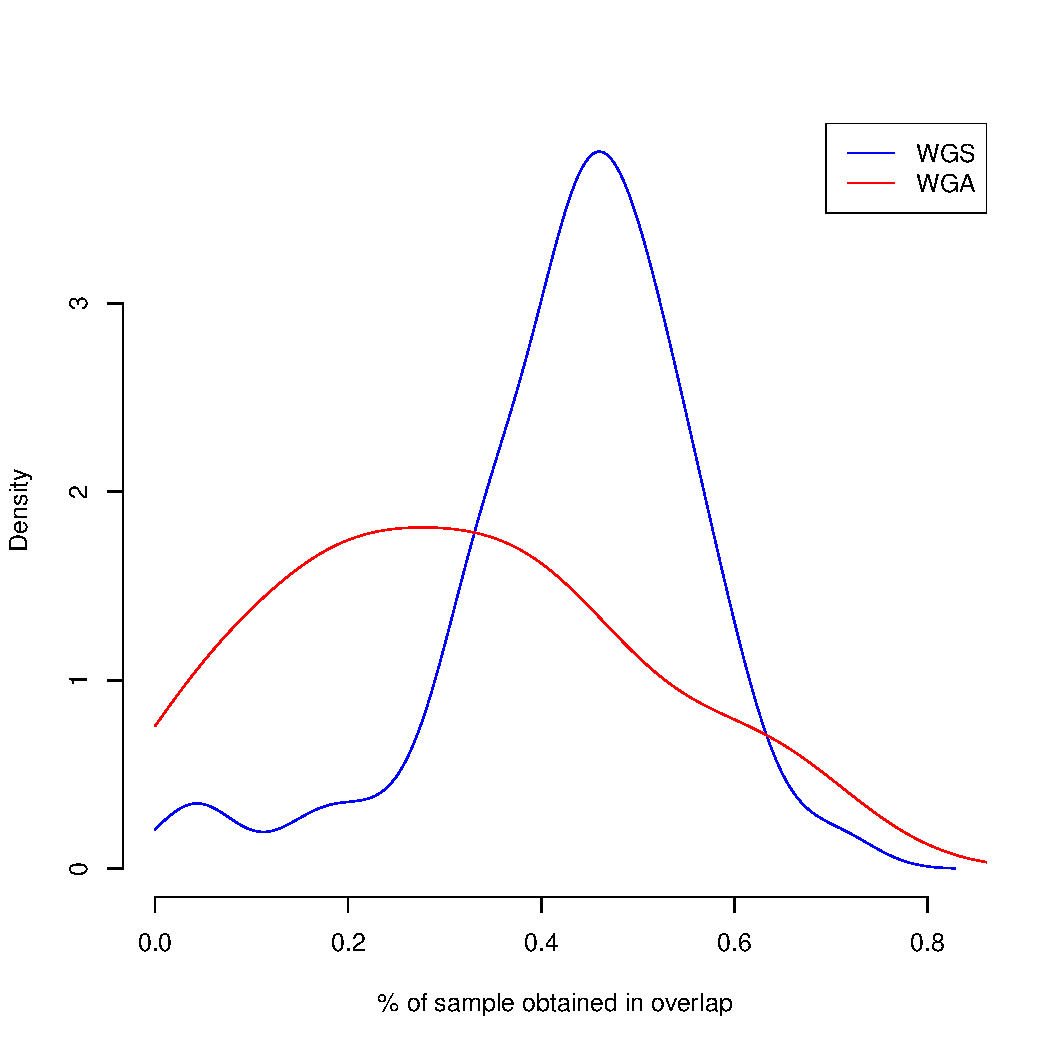
\includegraphics[width=5in]{unfiltered_overlap_WGS_WGA_together_densities.pdf} }
\caption{\textbf{Density of percentage overlap between WGS and WGA samples.} Density of the percentage of each WGS (blue) and WGA (red) sample that overlaps with the other sample from the same patient. The WGS distribution is higher and narrower, showing that the WGS samples overall have a higher percentage overlap than the WGA samples, and less range in this parameter. }
\end{figure}

%% Figure 5
\begin{figure}
\centerline{
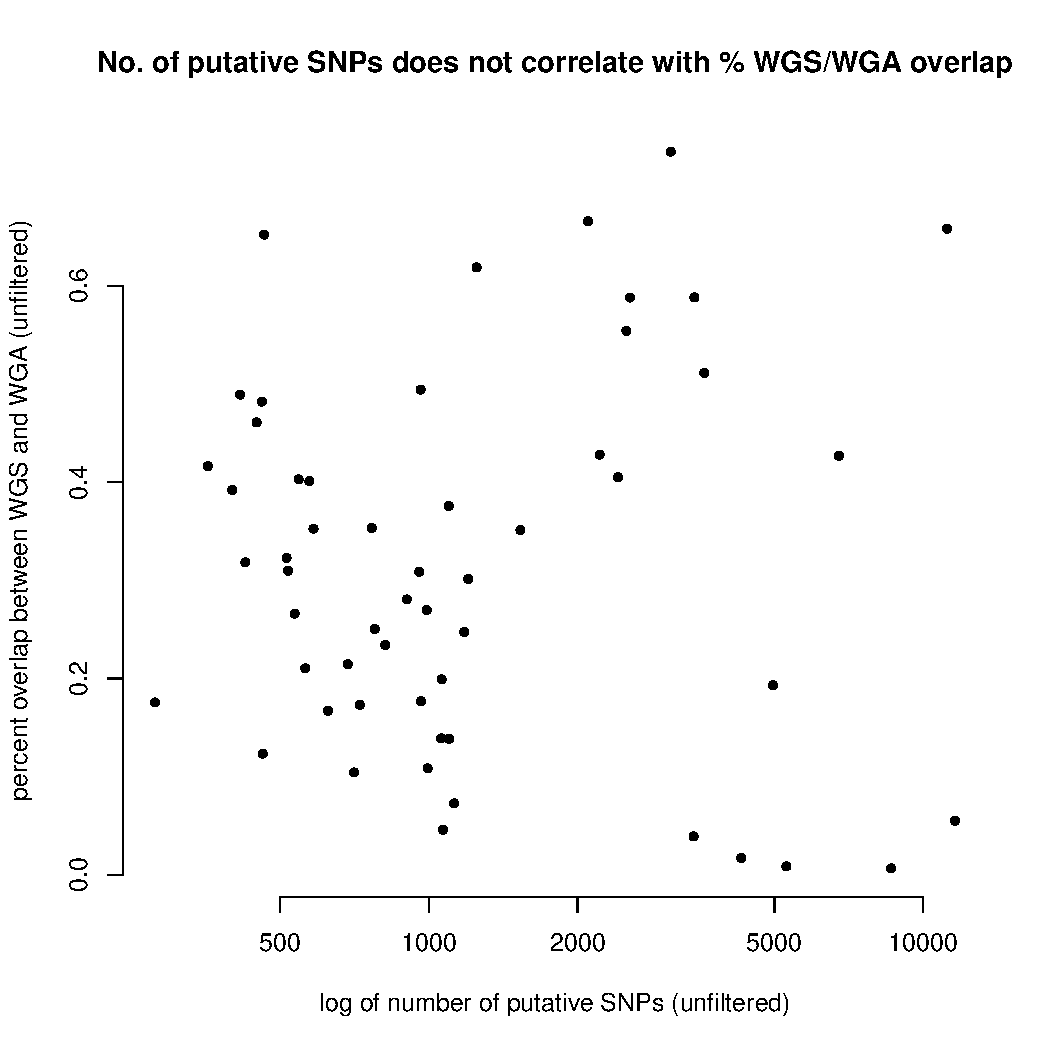
\includegraphics[width=5in]{unfiltered_total_muts_v_percent_overlap.pdf} }
\caption{\textbf{Percent of WGS/WGA overlap versus (log) number of putative SNPs per sample.} Plot of the percentage of the WGA samples that overlaped with the corresponding WGS samples (as a measure of sample quality) against the total number of putative SNPs in the WGS sample.}
\end{figure}

%% Figure 6
\begin{figure}
\centerline{
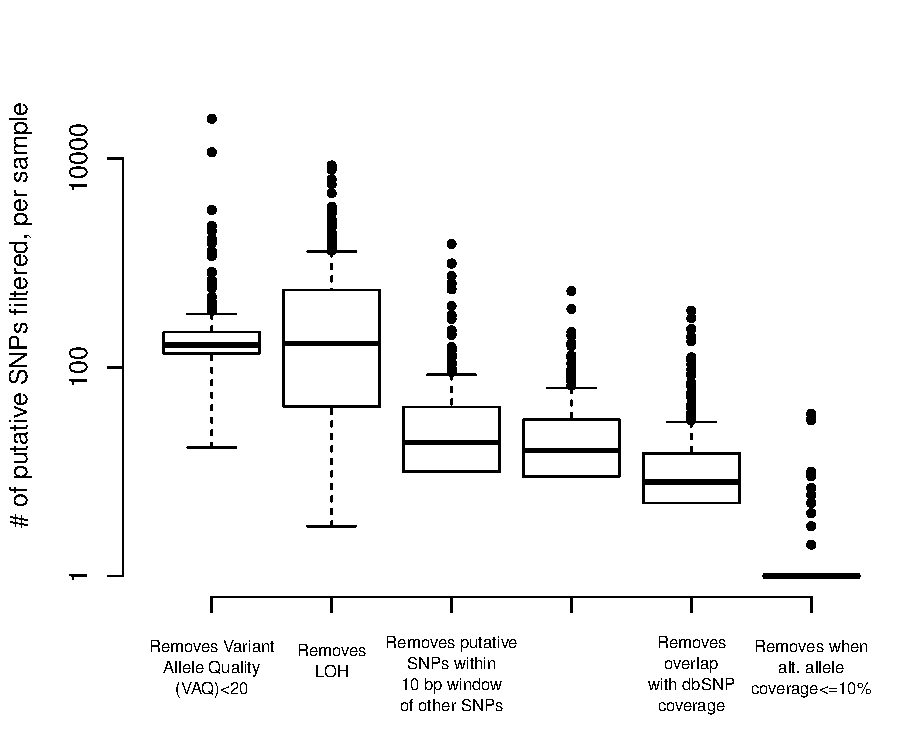
\includegraphics[width=6in]{boxplot_number_filtered.pdf} }
\caption{\textbf{Number of putative SNPs removed by each of six filters.} The $x-axis$ gives the name of those filters that removed putative SNPs, and the $y-axis$ gives, on a log scale, the number of mutations removed by a given filter in a given sample. Filters removing LOH and low VAQ putative SNPs removed around 100--200 putative SNPs on average. Three other filters, removing overlap with dbSNP and putative SNPs close to other putative mutations, removed on average about 50 mutations per sample.}
\end{figure}

%%Figure 7
\begin{figure}
% 379 samples, 311 patients
\centerline{
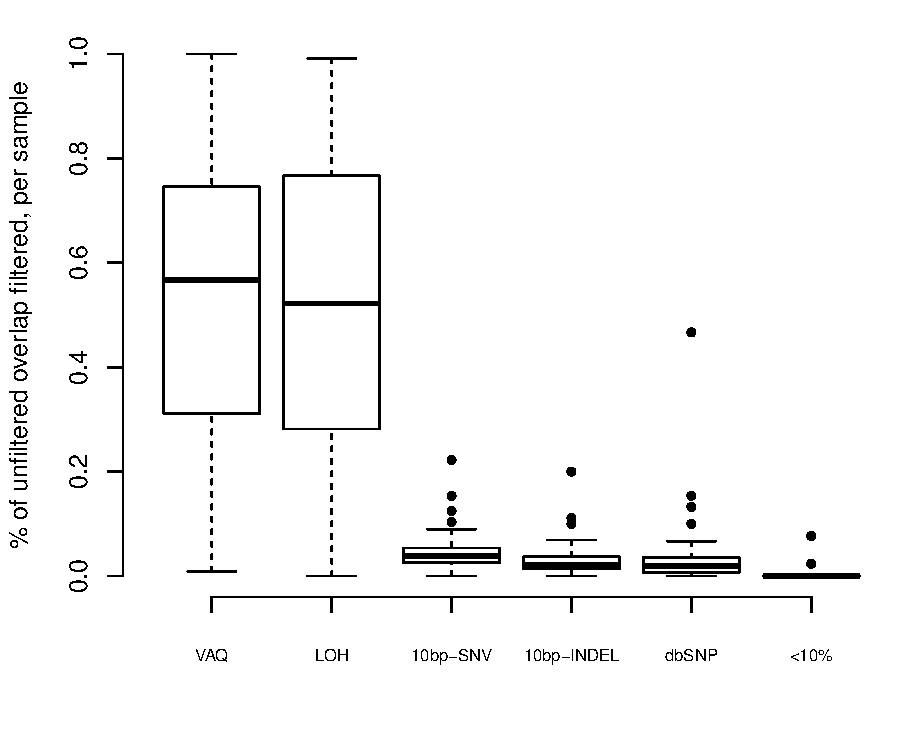
\includegraphics[width=6in]{boxplot_percent_overlap_filtered.pdf} }
\caption{\textbf{Percentage of WGS/WGA overlap removed, by filter.} The $x-axis$ describes the filters, and the $y-axis$ gives the percentage of the WGS/WGA overlap removed by the filter, per sample. Filters removing LOH and putative SNPs with low VAQ removed a significant percentage of the overlap; nothing else did.}
\end{figure}

%%Figure 8
\begin{figure}
\centerline{
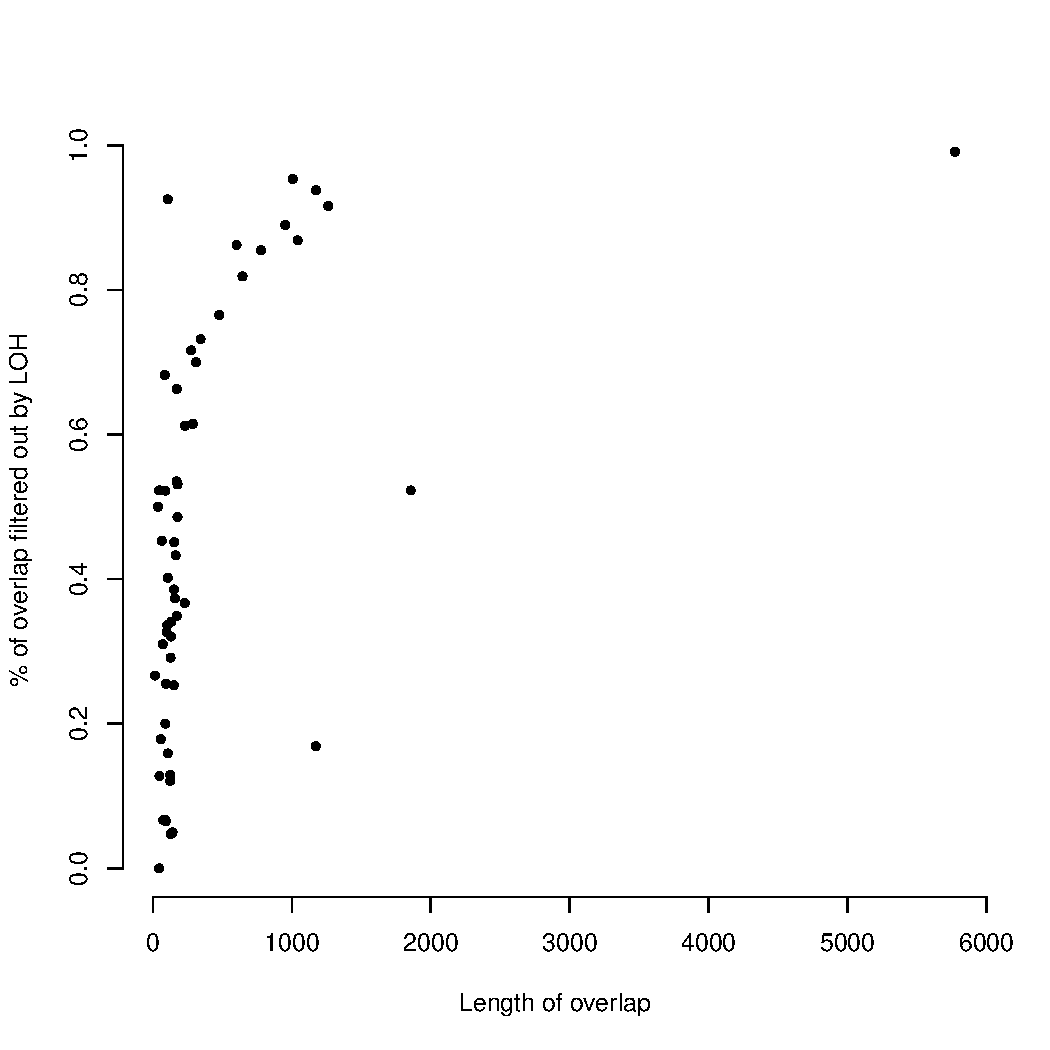
\includegraphics[width=5in]{./LOH_VAQ/LOH_all.pdf} }
\caption{\textbf{Length of overlap of LOH segments.} As the length of the overlap between WGS and WGA increases ($x-axis$), the number of mutations filtered out by LOH increases. This is the opposite of the pattern observed in VAQ mutations (Figure 6).}
\end{figure}

%%Figure 9
\begin{figure}
\centerline{
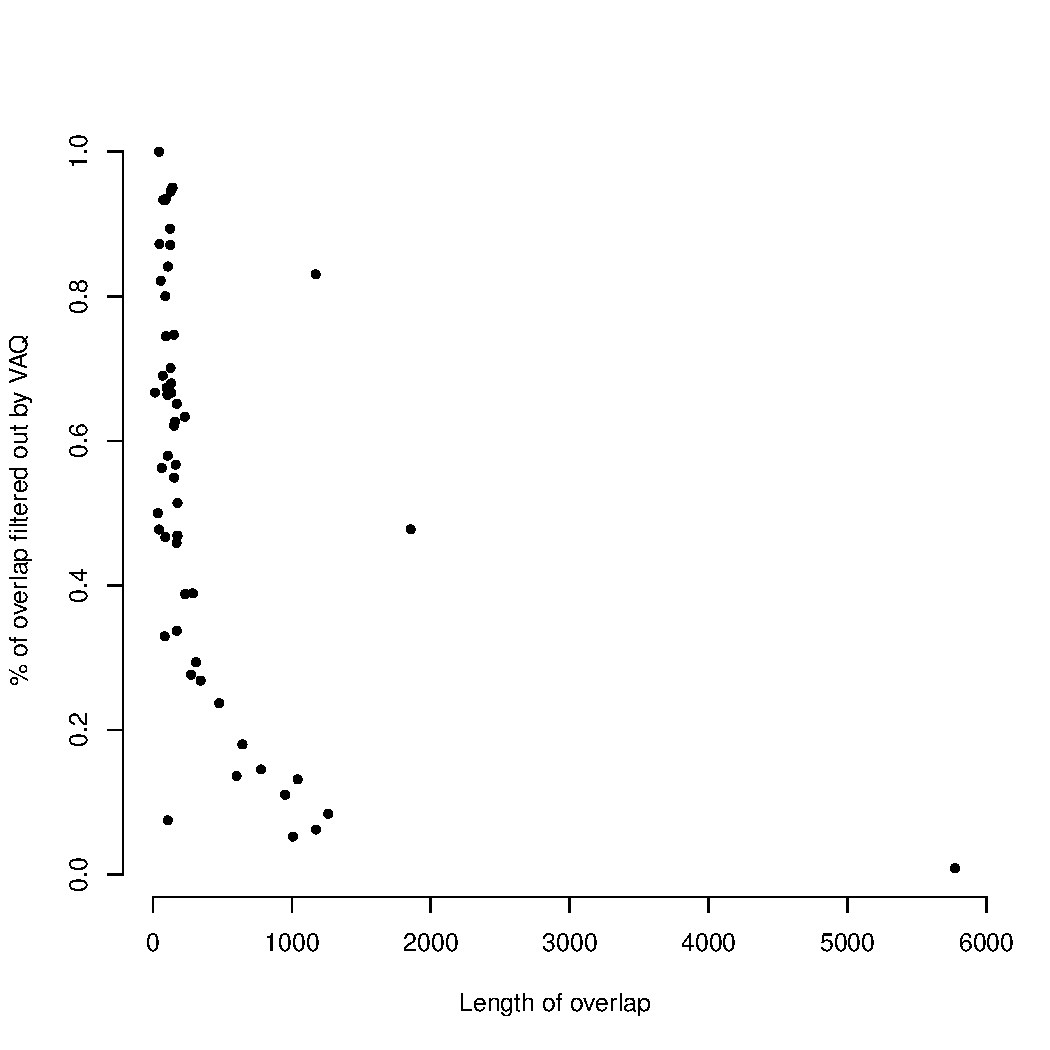
\includegraphics[width=5in]{./LOH_VAQ/VAQ_all.pdf} }
\caption{ \textbf{Length of overlap of VAQ segments.} As the length of the overlap between WGS and WGA increases ($x-axis$), the percentage of the overlap filtered out by VAQ decreases. This is the opposite of the pattern observed in LOH mutations (Figure 5).}
\end{figure}

\end{document}